\documentclass[tikz,border=3pt]{standalone}
\usepackage[T1]{fontenc}
\usepackage{lmodern}
\usetikzlibrary{arrows.meta,fit,positioning,backgrounds}

\definecolor{api}{HTML}{DCEAF5}
\definecolor{kubeml}{HTML}{CFE8F7}
\definecolor{kube}{HTML}{EEF1F3}
\definecolor{node}{HTML}{E5F2EA}
\definecolor{evidence}{HTML}{F4ECD7}
\definecolor{accent}{HTML}{1F77B4}
\definecolor{dark}{HTML}{263238}

\begin{document}
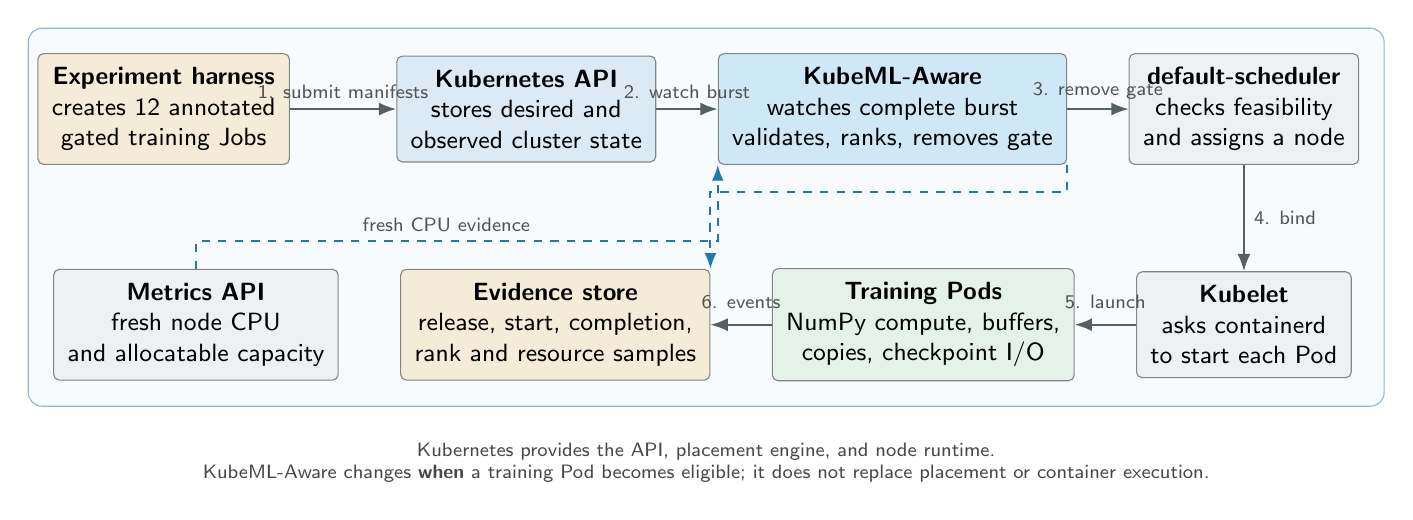
\begin{tikzpicture}[
  font=\sffamily\small,
  box/.style={draw=black!48, rounded corners=2pt, align=center, minimum height=1.05cm, inner sep=5pt},
  flow/.style={-{Latex[length=2.2mm]}, line width=0.75pt, draw=dark!78},
  feedback/.style={-{Latex[length=2mm]}, dashed, line width=0.7pt, draw=accent},
  label/.style={font=\sffamily\scriptsize, text=black!67, align=center}
]

\node[box,fill=evidence,minimum width=2.8cm] (submit) {
  \textbf{Experiment harness}\\
  creates 12 annotated\\
  gated training Jobs
};

\node[box,fill=api,minimum width=2.45cm,right=1.35cm of submit] (api) {
  \textbf{Kubernetes API}\\
  stores desired and\\
  observed cluster state
};

\node[box,fill=kubeml,minimum width=2.75cm,right=0.78cm of api] (controller) {
  \textbf{KubeML-Aware}\\
  watches complete burst\\
  validates, ranks, removes gate
};

\node[box,fill=kube,minimum width=2.35cm,right=0.78cm of controller] (scheduler) {
  \textbf{default-scheduler}\\
  checks feasibility\\
  and assigns a node
};

\node[box,fill=kube,minimum width=2.2cm,below=1.35cm of scheduler] (kubelet) {
  \textbf{Kubelet}\\
  asks containerd\\
  to start each Pod
};

\node[box,fill=node,minimum width=2.65cm,left=0.78cm of kubelet] (pods) {
  \textbf{Training Pods}\\
  NumPy compute, buffers,\\
  copies, checkpoint I/O
};

\node[box,fill=evidence,minimum width=2.35cm,left=0.78cm of pods] (records) {
  \textbf{Evidence store}\\
  release, start, completion,\\
  rank and resource samples
};

\node[box,fill=kube,minimum width=2.25cm,left=0.78cm of records] (metrics) {
  \textbf{Metrics API}\\
  fresh node CPU\\
  and allocatable capacity
};

\draw[flow] (submit) -- node[above,label]{1. submit manifests} (api);
\draw[flow] (api) -- node[above,label]{2. watch burst} (controller);
\draw[flow] (controller) -- node[above,label]{3. remove gate} (scheduler);
\draw[flow] (scheduler) -- node[right,label]{4. bind} (kubelet);
\draw[flow] (kubelet) -- node[above=2pt,label]{5. launch} (pods);
\draw[flow] (pods) -- node[above=2pt,label]{6. events} (records);
\draw[feedback] (metrics.north) -- ++(0,0.35) -|
  node[pos=0.24,above,label]{fresh CPU evidence} (controller.south west);
\draw[feedback] (controller.south east) -- ++(0,-0.34) -| (records.north east);

\begin{scope}[on background layer]
  \node[draw=accent!52,rounded corners=5pt,fill=accent!3,inner sep=9pt,
    fit=(api)(controller)(scheduler)(kubelet)(pods)(records)(metrics),
    label={[font=\sffamily\small\bfseries,text=accent]above:Single-node K3s cluster on the France VM}] (cluster) {};
\end{scope}

\node[below=0.34cm of cluster.south,font=\sffamily\scriptsize,text=black!72,align=center] {
  Kubernetes provides the API, placement engine, and node runtime.\\
  KubeML-Aware changes \textbf{when} a training Pod becomes eligible; it does not replace placement or container execution.
};

\end{tikzpicture}
\end{document}
